
In this section we will describe how we test the algorithms, and the testing framework.
\subsection{the transfer of analyses}

Our framework is shortly formulated in diagram \ref{fig:flowdiagram} where each node represents data/program.

\begin{figure}[t]
\center
\label{fig:flowdiagram}
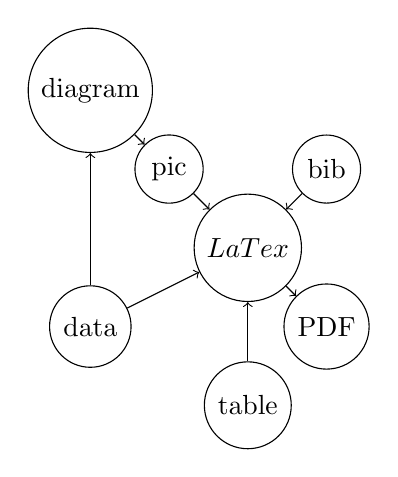
\begin{tikzpicture}
\node[draw,circle] at (0,0) (a) {$LaTex$};
\node[draw,circle] at (0,-2) (b) {table};
\node[draw,circle] at (-2,2) (c) {diagram};
\node[draw,circle] at (1,1) (d) {bib};
\node[draw,circle] at (-1,1) (e) {pic};
\node[draw,circle] at (-2,-1) (f) {data};
\node[draw,circle] at (1,-1) (g) {PDF};
\draw[->] (a) -- (g);
\draw[->] (d) -- (a);
\draw[->] (f) -- (a);
\draw[->] (b) -- (a);
\draw[->] (f) -- (c);
\draw[->] (c) -- (e);
\draw[->] (e) -- (a);
\end{tikzpicture}
\caption{This is the dataflow of the analyses}
\end{figure}

Everything is handled by a Makefile script\cite{olsen_files_nodate}. When we update a file, everything gets updated.

The plots generated by our scripts has the following conventions:
\begin{itemize}
	\item[-] The red area in the plots represent a 95\% confidence interval of the different times. The triangles represent the maximum and minimum values.
	\item[-] The 'Random' plots are completely random. Every iteration of every round are different to make sure that we can get an average case for the algorithm. 
\end{itemize}

\subsection{The testing process}

Our testing process follows a simple formula of every process is "perfect"\footnote{This is not true, but it is used as a principle to make it easier to divide up the work.}, and therefore let the script do its thing in good faith. This philosophy was created by Dennis Ritchie when developing UNIX\cite{ritchie_stream_1984}. To handle the inputs from each process we use a Makefile that is up to date on the files. 

